\documentclass{article}
\usepackage{CTEX}

%%%%%%%%%%%%%%%%%%%%%%%%%%%%%%%%%%%%%%%%%%%%%%%%%%%%%%%%%%%%%%%%%
\usepackage[a4paper]{geometry}
\geometry{left=3cm,right=3cm,top=3cm,bottom=3cm}
\linespread{1.5}
\usepackage{fancyhdr}

\usepackage{fontspec}
\defaultfontfeatures{Mapping=tex-text}
\usepackage{xunicode,xltxtra}
\usepackage[BoldFont,SlantFont,CJKnumber,CJKchecksingle]{xeCJK} \usepackage{CJKfntef}
\usepackage{bm} 
\usepackage{pifont}
\usepackage{color,xcolor}
\definecolor{GREEN}{RGB}{25,180,68}
\definecolor{YELLOW}{RGB}{255,255,224}
\definecolor{BLUE}{RGB}{65,105,225}
\definecolor{RED}{RGB}{139,0,0}
\definecolor{DRED}{RGB}{128,0,0}
\definecolor{GREY}{RGB}{128,128,128}

\usepackage{amsmath,amsfonts,amssymb}

\usepackage[americaninductors,europeanresistors]{circuitikz}
\usepackage{tikz}
\usetikzlibrary{positioning,arrows,shadows,shapes,calc,mindmap,trees,backgrounds}
\usepackage{graphicx}
\usepackage{subfigure} 
\usepackage{colortbl,dcolumn}  
\usepackage{multirow}
\usepackage{multicol}
\usepackage{booktabs}
\usepackage{fancyvrb}
\usepackage{listings}

\usepackage{titlesec}
\usepackage{etoolbox}
\makeatletter
\patchcmd{\ttlh@hang}{\parindent\z@}{\parindent\z@\leavevmode}{}{}
\patchcmd{\ttlh@hang}{\noindent}{}{}{}
\makeatother
\usepackage{mdwlist}
\usepackage{verbatim}
\usepackage{/Users/jinna/styles/zhfontcfg}
\usepackage{/Users/jinna/styles/visionouclistings}
\usepackage{/Users/jinna/styles/visionouccfg}
\setlength{\headheight}{15pt}
\fancyhf{}
\setCJKmainfont{Adobe Kaiti Std} 
\setCJKmonofont{Adobe Fangsong Std}
\makeatletter
\def\headrule{{\if@fancyplain\let\headrulewidth\plainheadrulewidth\fi%
\color{BLUE}
\hrule\@height 2.5pt \@width\headwidth\vskip1pt 
\hrule\@height 0.5pt\@width\headwidth              
\vskip-2\headrulewidth\vskip-1pt}        
\vspace{6mm}}                
\makeatother         

\graphicspath{{figures/}}
\tikzset{
    >=stealth',
    punkt/.style={
           rectangle,
           rounded corners,
           draw=black, very thick,
           text width=6.5em,
           minimum height=2em,
           text centered},
    pil/.style={
           ->,
           thick,
           shorten <=2pt,
           shorten >=2pt,},
    FlyZhyBall/.style={
      circle,
      minimum size=6mm,
      inner sep=0.5pt,
      ball color=red!50!blue,
      text=white,},
    FlyZhyRectangle/.style={
      rectangle,
      rounded corners,
      minimum size=6mm,
      ball color=red!50!blue,
      text=white,},
    zhyfly/.style={
      rectangle,
      rounded corners,
      minimum size=6mm,
      ball color=red!25!blue,
      text=white,},
    nrectangle/.style={
      rectangle,
      draw=#1!50,
      fill=#1!20,
      minimum size=5mm,
      inner sep=0.1pt,}
}

% code
\lstnewenvironment{VHDLcode}[1][]{%
  \lstset{
    basicstyle=\footnotesize\ttfamily\color{black},%
    columns=flexible,%
    framexleftmargin=.7mm,frame=shadowbox,%
    rulesepcolor=\color{blue},%
%    frame=single,%
    backgroundcolor=\color{yellow!20},%
    xleftmargin=1.2\fboxsep,%
    xrightmargin=.7\fboxsep,%
    numberstyle=\tiny\color{blue},%
    numberblanklines=false,numbersep=7pt,%
    language=VHDL%
    }\lstset{#1}}{}
\lstnewenvironment{VHDLmiddle}[1][]{%
  \lstset{
    basicstyle=\scriptsize\ttfamily\color{black},%
    columns=flexible,%
    framexleftmargin=.7mm,frame=shadowbox,%
    rulesepcolor=\color{blue},%
%    frame=single,%
    backgroundcolor=\color{yellow!20},%
    xleftmargin=1.2\fboxsep,%
    xrightmargin=.7\fboxsep,%
    numbers=left,numberstyle=\tiny\color{blue},%
    numberblanklines=false,numbersep=7pt,%
    language=VHDL%
    }\lstset{#1}}{}
\lstnewenvironment{VHDLsmall}[1][]{%
  \lstset{
    basicstyle=\tiny\ttfamily\color{black},%
    columns=flexible,%
    framexleftmargin=.7mm,frame=shadowbox,%
    rulesepcolor=\color{blue},%
%    frame=single,%
    backgroundcolor=\color{yellow!20},%
    xleftmargin=1.2\fboxsep,%
    xrightmargin=.7\fboxsep,%
    numbers=left,numberstyle=\tiny\color{blue},%
    numberblanklines=false,numbersep=7pt,%
    language=VHDL%
    }\lstset{#1}}{}
% pdf
\hypersetup{pdfauthor={Haiyong Zheng},%
            pdftitle={Title},%
            CJKbookmarks=true,%
            bookmarksnumbered=true,%
            bookmarksopen=false,%
            plainpages=false,%
            colorlinks=true,%
            citecolor=green,%
            filecolor=magenta,%
            linkcolor=DRED,%red(default)
            urlcolor=cyan}
\newcommand\titlebar{%
\tikz[baseline,trim left=3.1cm,trim right=3cm] {
    \fill [cyan!25] (2.5cm,-1ex) rectangle (\textwidth+3.1cm,2.5ex);
    \node [
        fill=cyan!60!white,
        anchor= base east,
        rounded rectangle,
        minimum height=3.5ex] at (3cm,0) {
        \textbf{\thesection.}
    };
}%
}

\definecolor{mygreen}{rgb}{0,0.6,0}
\definecolor{mygray}{rgb}{0.5,0.5,0.5}
\definecolor{mymauve}{rgb}{0.58,0,0.82}
\lstset{
 backgroundcolor=\color{white}, 
 basicstyle = \footnotesize,       
 breakatwhitespace = false,        
 breaklines = true,                 
 captionpos = b,                    
 commentstyle = \color{mygreen}\bfseries,
 extendedchars = false,             
 frame =shadowbox, 
 framerule=0.5pt,
 keepspaces=true,
 keywordstyle=\color{blue}\bfseries, % keyword style
 language = C++,                     % the language of code
 otherkeywords={string}, 
 numbers=left, 
 numbersep=5pt,
 numberstyle=\tiny\color{mygray},
 rulecolor=\color{black},         
 showspaces=false,  
 showstringspaces=false, 
 showtabs=false,    
 stepnumber=1,         
 stringstyle=\color{mymauve},        % string literal style
 tabsize=2,          
 title=\lstname                      
}


%%%%%%%%%%%%%%%%%%%%%%%%%%%%%%%%%%%%%%%%%%%%%%%%%%%%%%%%%%%
%设置标题页面               
\chead{\color{GREY}Experiment Report}%页眉
\cfoot{\color{GREY}12.11}%页脚 中
\lfoot{\color{GREY}Jinna}%页脚 左
\rfoot{\color{GREY}\thepage\ }%页脚 右
\renewcommand{\headrulewidth}{0.4pt}
\renewcommand{\footrulewidth}{0.4pt}
\usepackage{/Users/jinna/styles/lshort}

%%%%%%%%%%%%%%%%%%%%%%%%%%%%%%%%%%%%%%%%%%%%%%%%%%%%%%%%%%%%%%%%%
\begin{document}

\pagenumbering{roman}


\pagestyle{fancy}
%%%%%%%%%%%%%%%%%%%%%%%%%%%%%%%%%%%%%%%%%%%%%%%%%%%%%%%%%%%%%%%%%
\begin{center}
\textbf{\LARGE{Experiment Report}} %标题加黑加大居
\end{center}

\begin{center}
Jinna Cui
\end{center}

\begin{center}
01.02-01.08
\end{center}
These two weeks, I mainly focus on experiments. I did many experiments on the database. Firstly, I trained on 98classes of WHOI 2013 images, and test on 98 classes of WHOI 2014 images. Mix class is deleted firstly because of the huge amount and the processing speed is too slow. The other four classes are deleted because these four classes are empty in 2013 database but not empty in 2014 database, also means that these four classes are empty in training database but not empty in test database. So I deleted these four classes. Secondly, after the processing of mix class finished, I started to do experiment on 103 classes. I also add four classes which are deleted before into the training database and test database again. Because these four classes images are less than 100, and what we need is the accuracy improvement from one-single channel network to three-channel network. So I think I can use all the 2013 images as training database and all the 2014 images as test database. 
\section{The experiment on 98 classes database}
The local feature images are get by bilateral filtering and the local feature images are get by Gaussian high-pass filtering and logarithmic enhancement. The accuracy is overall accuracy. 

\begin{table}[!ht]
  \caption{Accuracy of Plankton Classification}
  \centering
  \begin{tabular}{lllll}
    \toprule
    \cmidrule{1-5}
    training database &test database &network  &input data   &accuracy  \\
    \midrule
    WHOI2013 98classes &WHOI2014 98 classes & one-channel AlexNet &original images   & 87.51\% \\ \hline
    WHOI2013 98classes &WHOI2014 98 classes  &one-channel  AlexNet &local-feature images & 88.11\%  \\ \hline
    WHOI2013 98classes &WHOI2014 98 classes  &one-channel  AlexNet &global-feature images   & 81.95\% \\ \hline
    WHOI2013 98classes &WHOI2014 98 classes  &three-channel  AlexNet &original\&local\&global images   & 88.04\% \\
    \bottomrule
  \end{tabular}
\end{table}

\begin{figure}[!ht] 
  \centering 
  \subfigure[Training loss of one-channel AlexNet on original images]{ 
    \label{fig:subfig:a} %% label for first subfigure 
    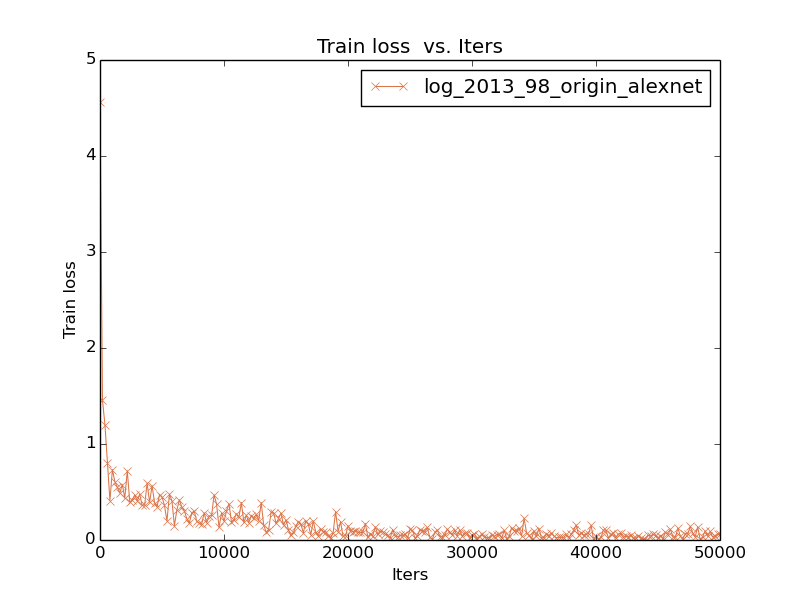
\includegraphics[width=5cm,height=5cm]{1.png}} 
  \hspace{0.3in} 
  \subfigure[Training loss of three-channel AlexNet on original\&local feature\&global feature images]{ 
    \label{fig:subfig:b} %% label for second subfigure 
    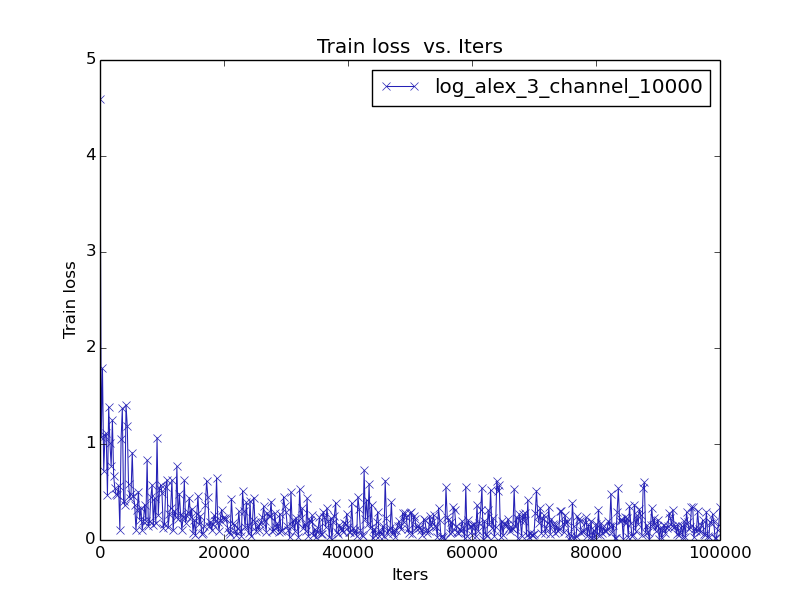
\includegraphics[width=5cm,height=5cm]{2.png}} 
   \hspace{0.3in} 
\end{figure}

In Dai Jialun's paper, he just adds meanfile on original images in 3-channel network. He didn't add meanfile on the channel of local feature images channel and global feature images channel. But in my first experiment, I add meanfile on three channels, so I also do an experiment with only one meanfile original images channel. 

\begin{table}[!ht]
  \caption{Accuracy of Plankton Classification}
  \centering
  \begin{tabular}{lllll}
    \toprule
    \cmidrule{1-5}
  	database &network  &input data   &accuracy  \\
    \midrule
    WHOI2013&2014 98classes  &one-channel  AlexNet &original\&local\&global images with three meanfiles   & 88.04\% \\ \hline
    WHOI2013&2014 98classes   &three-channel  AlexNet &original\&local\&global images  with one meanfile  &87.99\% \\
    \bottomrule
  \end{tabular}
\end{table}

\begin{figure}[!ht] 
  \centering 
  \subfigure[Training loss of three-channel AlexNet with three meanfiles]{ 
    \label{fig:subfig:a} %% label for first subfigure 
    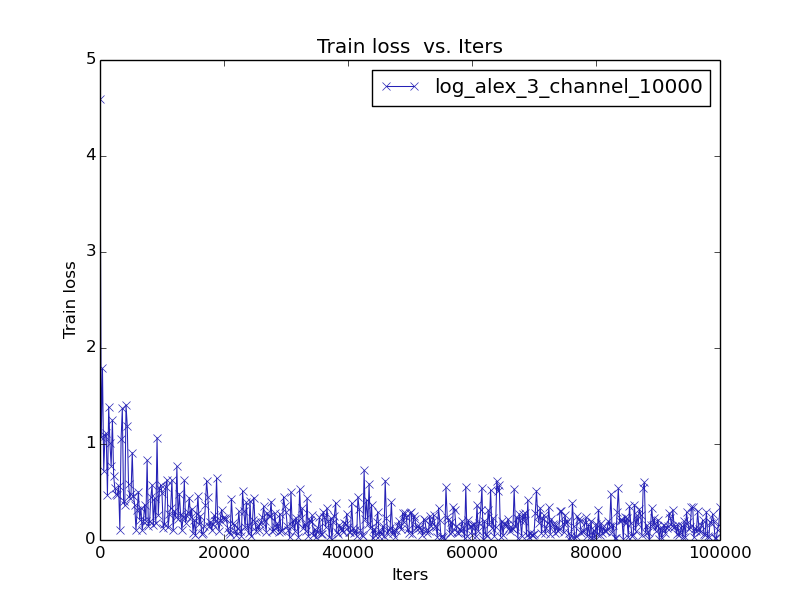
\includegraphics[width=5cm,height=5cm]{2.png}} 
  \hspace{0.3in} 
  \subfigure[Training loss of three-channel AlexNet with one meanfile]{ 
    \label{fig:subfig:b} %% label for second subfigure 
    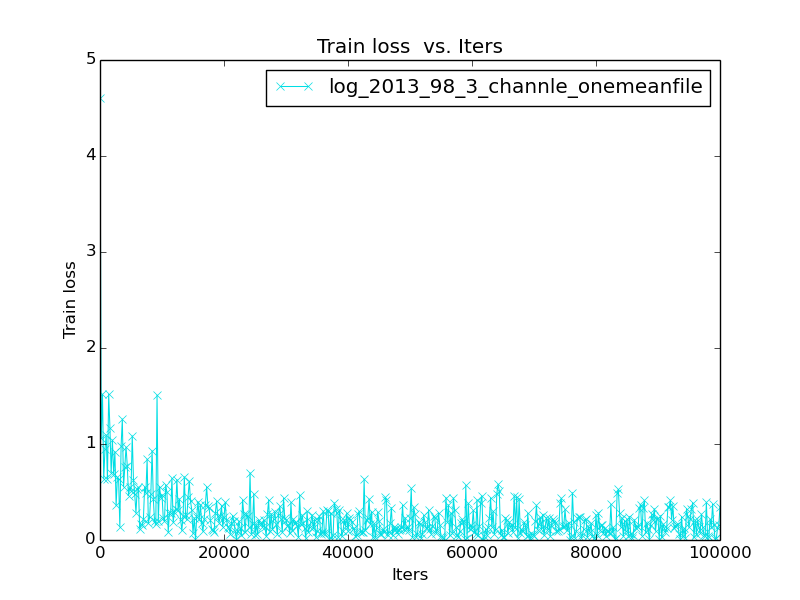
\includegraphics[width=5cm,height=5cm]{3.png}} 
   \hspace{0.3in} 
\end{figure}
\section{The experiment on 103 classes database}
\begin{table}[!ht]
  \caption{Accuracy of Plankton Classification}
  \centering
  \begin{tabular}{lllll}
    \toprule
    \cmidrule{1-5}
    training database &test database &network  &input data   &accuracy  \\
    \midrule
    WHOI2013 98classes &WHOI2014 103 classes & one-channel AlexNet &original images   & 93.17\% \\ \hline
    WHOI2013 98classes &WHOI2014 103 classes  &one-channel  AlexNet &local-feature images & 93.63\%  \\ \hline
    WHOI2013 98classes &WHOI2014 103 classes  &one-channel  AlexNet &global-feature images   & 90.29\% \\ \hline
    WHOI2013 98classes &WHOI2014 103 classes  &three-channel  AlexNet &original\&local\&global images   & 93.10\% \\
    \bottomrule
  \end{tabular}
\end{table}

In the experiment we can see that, the bilateral filtering to get global feature method didn't get better overall accuracy.  

\end{document}